\subsection{Completed ablation loss trajectories}
Each panel uses one predeclared fixed learning rate and only full-budget completed runs. The ablation matrix may still be incomplete; missing variants are not assigned values. All completed variants, including adverse ones, are retained.
\begin{figure}[!htbp]
\centering
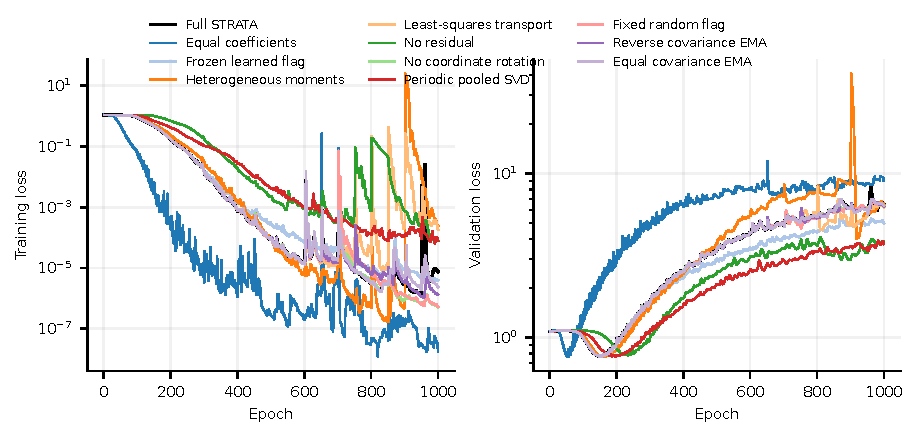
\includegraphics[width=.98\linewidth]{figures/fig_ablation_complete_f4222fea23ff.pdf}
\caption{\textbf{Completed fixed-rate ablation trajectories.} PubMed/sage/64/0.0003. Left: training; right: validation. Raw losses for the full method and every currently completed variant, seed 42. No smoothing, test selection or extrapolation. In continual learning the validation set averages seen tasks.}
\end{figure}
\begin{figure}[!htbp]
\centering
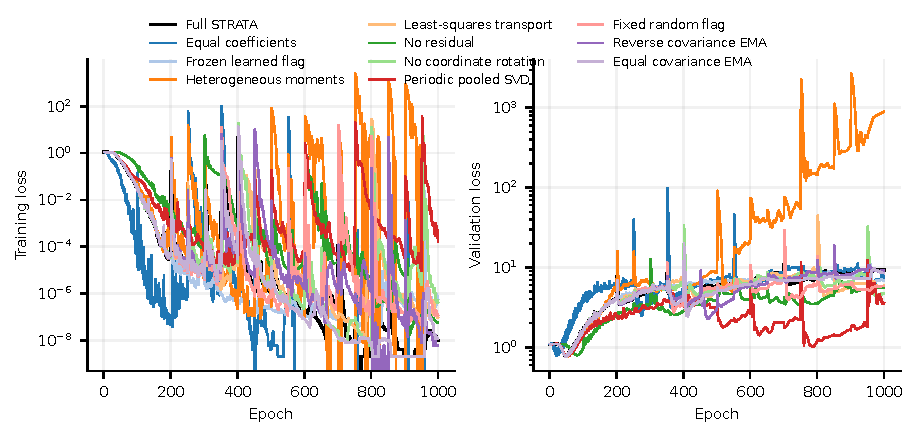
\includegraphics[width=.98\linewidth]{figures/fig_ablation_complete_92ad161e923b.pdf}
\caption{\textbf{Completed fixed-rate ablation trajectories.} PubMed/sage/64/0.001. Left: training; right: validation. Raw losses for the full method and every currently completed variant, seed 42. No smoothing, test selection or extrapolation. In continual learning the validation set averages seen tasks.}
\end{figure}
\begin{figure}[!htbp]
\centering
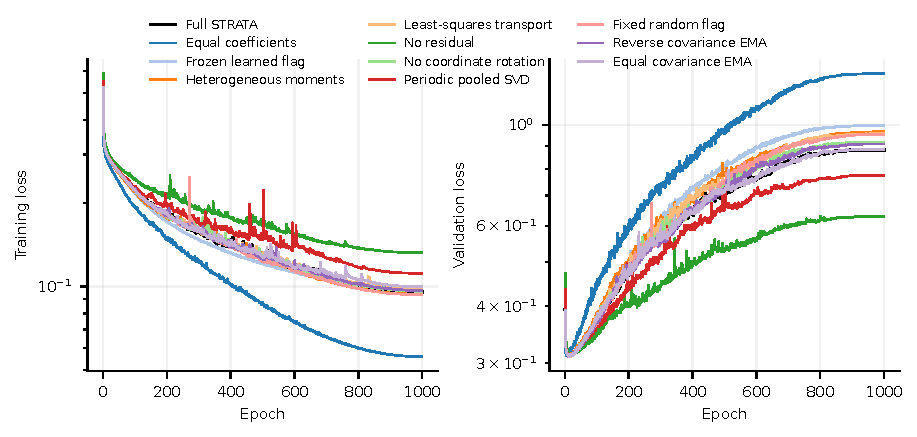
\includegraphics[width=.98\linewidth]{figures/fig_ablation_complete_cd63c9d43c42.pdf}
\caption{\textbf{Completed fixed-rate ablation trajectories.} adult/MLP-256-256/64/0.0003. Left: training; right: validation. Raw losses for the full method and every currently completed variant, seed 42. No smoothing, test selection or extrapolation. In continual learning the validation set averages seen tasks.}
\end{figure}
\begin{figure}[!htbp]
\centering
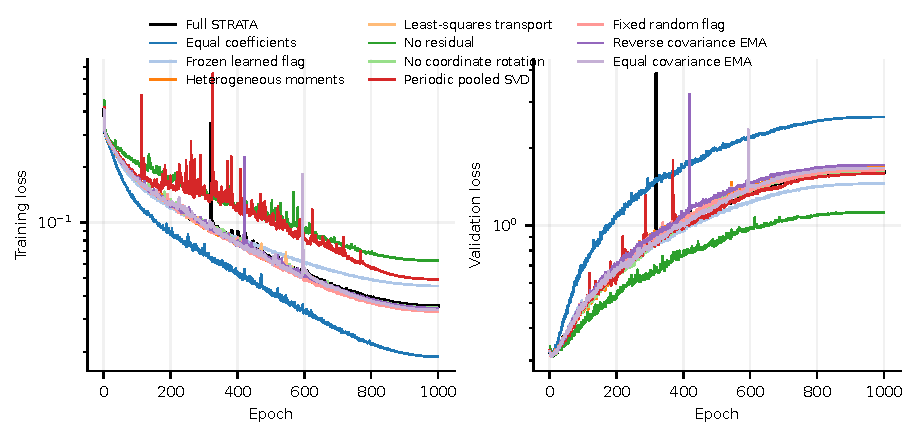
\includegraphics[width=.98\linewidth]{figures/fig_ablation_complete_f1b02595ebb0.pdf}
\caption{\textbf{Completed fixed-rate ablation trajectories.} adult/MLP-256-256/64/0.001. Left: training; right: validation. Raw losses for the full method and every currently completed variant, seed 42. No smoothing, test selection or extrapolation. In continual learning the validation set averages seen tasks.}
\end{figure}
\begin{figure}[!htbp]
\centering
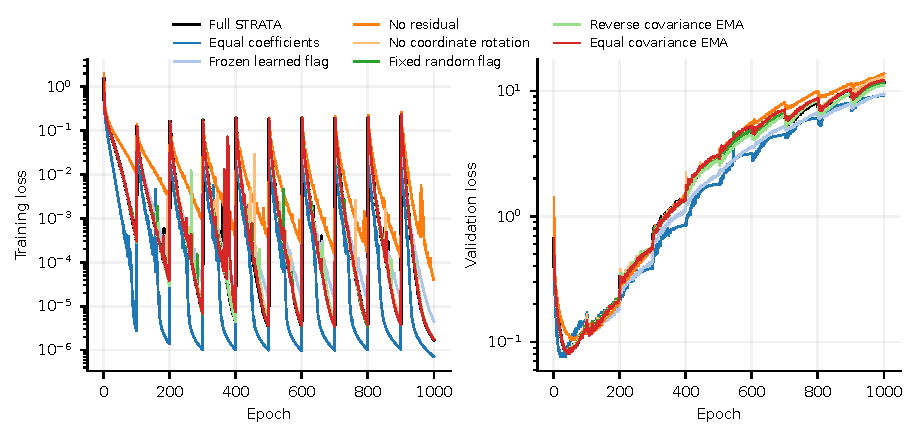
\includegraphics[width=.98\linewidth]{figures/fig_ablation_complete_22095cc4347a.pdf}
\caption{\textbf{Completed fixed-rate ablation trajectories.} rotated\_mnist\_cl/MLP-256-256/64/0.0003. Left: training; right: validation. Raw losses for the full method and every currently completed variant, seed 42. No smoothing, test selection or extrapolation. In continual learning the validation set averages seen tasks.}
\end{figure}
\begin{figure}[!htbp]
\centering
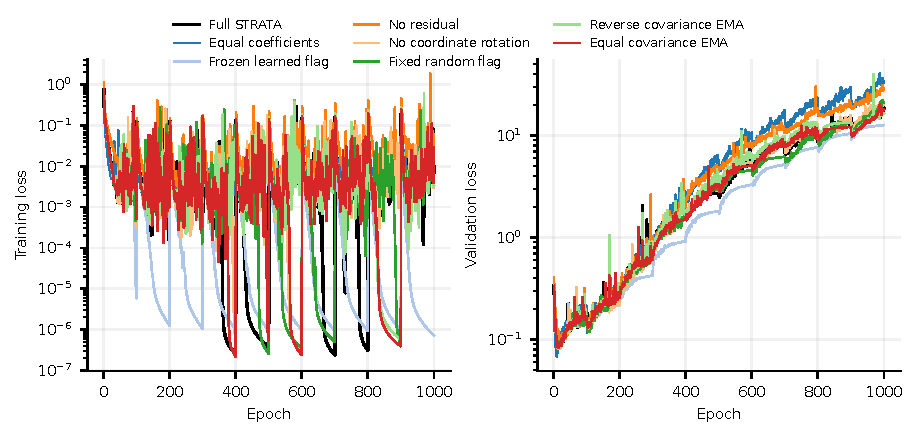
\includegraphics[width=.98\linewidth]{figures/fig_ablation_complete_4cf87464d8ba.pdf}
\caption{\textbf{Completed fixed-rate ablation trajectories.} rotated\_mnist\_cl/MLP-256-256/64/0.001. Left: training; right: validation. Raw losses for the full method and every currently completed variant, seed 42. No smoothing, test selection or extrapolation. In continual learning the validation set averages seen tasks.}
\end{figure}
\begin{figure}[!htbp]
\centering
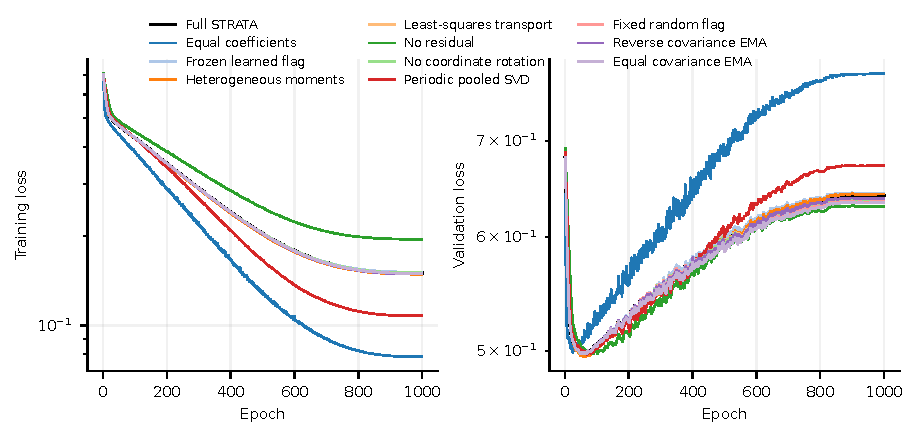
\includegraphics[width=.98\linewidth]{figures/fig_ablation_complete_6327e4845709.pdf}
\caption{\textbf{Completed fixed-rate ablation trajectories.} wine\_red/MLP-256-256/64/0.0003. Left: training; right: validation. Raw losses for the full method and every currently completed variant, seed 42. No smoothing, test selection or extrapolation. In continual learning the validation set averages seen tasks.}
\end{figure}
\begin{figure}[!htbp]
\centering
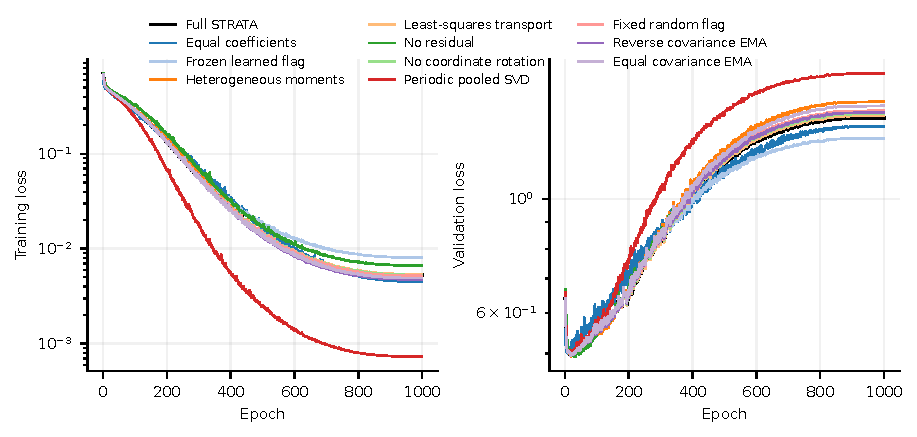
\includegraphics[width=.98\linewidth]{figures/fig_ablation_complete_f7dd6296b414.pdf}
\caption{\textbf{Completed fixed-rate ablation trajectories.} wine\_red/MLP-256-256/64/0.001. Left: training; right: validation. Raw losses for the full method and every currently completed variant, seed 42. No smoothing, test selection or extrapolation. In continual learning the validation set averages seen tasks.}
\end{figure}
